\documentclass[12pt,letterpaper]{exam}
\usepackage[lmargin=1in,rmargin=1in,tmargin=1in,bmargin=1in]{geometry}
\usepackage{../style/exams}

% -------------------
% Course & Exam Information
% -------------------
\newcommand{\course}{MAT 108: Exam 3}
\renewcommand{\term}{Spring -- 2022}
\newcommand{\examdate}{05/11/2022}
\newcommand{\timelimit}{85 Minutes}

\setbool{hideans}{true} % Student: True; Instructor: False

% -------------------
% Content
% -------------------
\begin{document}

\examtitle
\instructions{Write your name on the appropriate line on the exam cover sheet. This exam contains \numpages\ pages (including this cover page) and \numquestions\ questions. Check that you have every page of the exam. Answer the questions in the spaces provided on the question sheets. Be sure to answer every part of each question and show all your work. If you run out of room for an answer, continue on the back of the page --- being sure to indicate the problem number.} 
\scores
\bottomline
\newpage

% ---------
% Questions
% ---------
\begin{questions}

% Question 1
\newpage
\question A student is given a set of data points on an exam to for which they are to create a linear regression. Suppose that the points are $(-2, 1)$, $(0, 5)$, $(2, 3)$, and $(4, 5)$. Their computation of the least square regression line is shown below. Unfortunately, they spilled coffee on their work, obscuring some of the numbers. 

\begin{parts}
\part[7] Recompute (i)--(vii) for the student and place your answers in the appropriate space below. 
	\[
	\begin{aligned}
	\overline{x}&= \text{(i)} \\[0.3cm]
	\overline{y}&= \dfrac{1 + 5 + 3 + 5}{4}= \dfrac{14}{4}= 3.5 \\[0.3cm]
	s_x^2&= \dfrac{1}{3} \cdot 20 \approx 6.6667 \Longrightarrow s_x \approx 2.582 \\[0.3cm]
	s_y^2&= \text{(ii)} \Longrightarrow s_y= \text{(iii)}
	\end{aligned}
	\]
	
\begin{table}[!ht]
\centering
\begin{tabular}{rrrrrrrrr}
\multicolumn{1}{c|}{$x$} & \multicolumn{1}{c|}{$y$} & \multicolumn{1}{c|}{$x_i - \overline{x}$} & \multicolumn{1}{c|}{$(x_i - \overline{x})^2$} & \multicolumn{1}{c|}{$y_i - \overline{y}$} & \multicolumn{1}{c|}{$(y_i - \overline{y})^2$} & \multicolumn{1}{c|}{$\frac{x_i - \overline{x}}{s_x}$} & \multicolumn{1}{c|}{$\frac{y_i - \overline{y}}{s_y}$} & \multicolumn{1}{c}{$\frac{x_i - \overline{x}}{s_x} \cdot \frac{y_i - \overline{y}}{s_y}$} \\ \hline
\multicolumn{1}{r|}{$-2$} & \multicolumn{1}{r|}{$1$} & \multicolumn{1}{r|}{(iv)} & \multicolumn{1}{r|}{$9$} & \multicolumn{1}{r|}{$-2.5$} & \multicolumn{1}{r|}{$6.25$} & \multicolumn{1}{r|}{$-1.1619$} & \multicolumn{1}{r|}{$-1.3056$} & $1.517$ \\
\multicolumn{1}{r|}{$0$} & \multicolumn{1}{r|}{$5$} & \multicolumn{1}{r|}{$-1$} & \multicolumn{1}{r|}{$1$} & \multicolumn{1}{r|}{$1.5$} & \multicolumn{1}{r|}{$2.25$} & \multicolumn{1}{r|}{$-0.3873$} & \multicolumn{1}{r|}{$0.7833$} & $-0.3034$ \\
\multicolumn{1}{r|}{$2$} & \multicolumn{1}{r|}{$3$} & \multicolumn{1}{r|}{$1$} & \multicolumn{1}{r|}{$1$} & \multicolumn{1}{r|}{$-0.5$} & \multicolumn{1}{r|}{(v)} & \multicolumn{1}{r|}{$0.3873$} & \multicolumn{1}{r|}{$-0.2611$} & $-0.1011$ \\
\multicolumn{1}{r|}{$4$} & \multicolumn{1}{r|}{$5$} & \multicolumn{1}{r|}{$3$} & \multicolumn{1}{r|}{$9$} & \multicolumn{1}{r|}{$1.5$} & \multicolumn{1}{r|}{$2.25$} & \multicolumn{1}{r|}{$1.1619$} & \multicolumn{1}{r|}{$0.7833$} & (vi) \\ \hline
\multicolumn{1}{l}{} & \multicolumn{1}{l}{} & Sum: & (vii) & Sum: & $11$ & \multicolumn{1}{l}{} & Sum: & $2.0226$
\end{tabular}
\end{table}

	\[
	\begin{aligned}
	\text{(i)}&= & \hspace{8cm} && \text{(v)}&= \phantom{xxxxxxxxxxxxx} \\[0.3cm]
	\text{(ii)}&= & && \text{(vi)}&= \\[0.3cm]
	\text{(iii)}&= & && \text{(vii)}&= \\[0.3cm]
	\text{(iv)}&= 
	\end{aligned}
	\]

\part[5] Compute $r^2$ for the student. Based on this value, explain to the student whether the least square regression line is a `good' model. \vfill

\part[4] Given that the resulting linear regression is $\widehat{y}= 0.5x + 3$, find the predicted value for $x= 2$ and its corresponding residual for the student. \vfill
\end{parts}



% Question 2
\newpage
\question[8] The same student from Problem~1 also had to compute the regression coefficient, $R$, for several different data sets. Unfortunately, they dropped their papers---separating the data from the computed $R$ value. Match the dataset to the most likely regression coefficient for the student. \pspace
	\begin{figure}[!ht]
	\centering
	\begin{minipage}{0.45\textwidth}
	   \centering
	   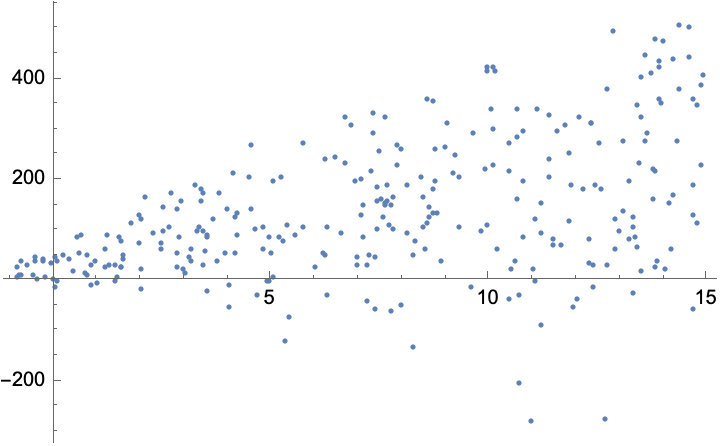
\includegraphics[width=0.9\textwidth]{reg1.png}
	   \caption*{(a)}
	\end{minipage}\hfill
	\begin{minipage}{0.45\textwidth}
	   \centering
	   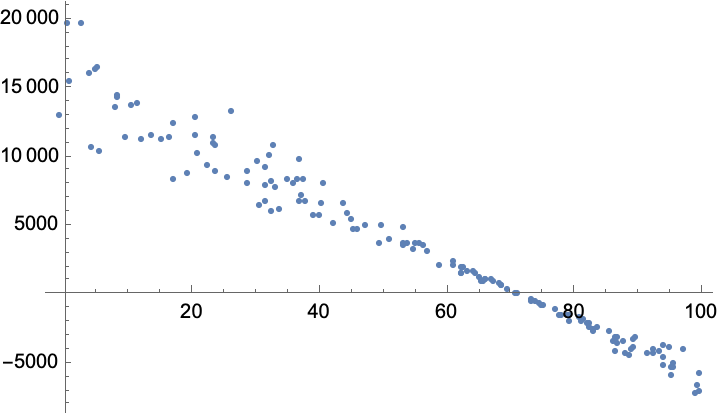
\includegraphics[width=0.9\textwidth]{reg2.png}
	   \caption*{(b)}
	\end{minipage}
	\begin{minipage}{0.45\textwidth}
	   \centering
	   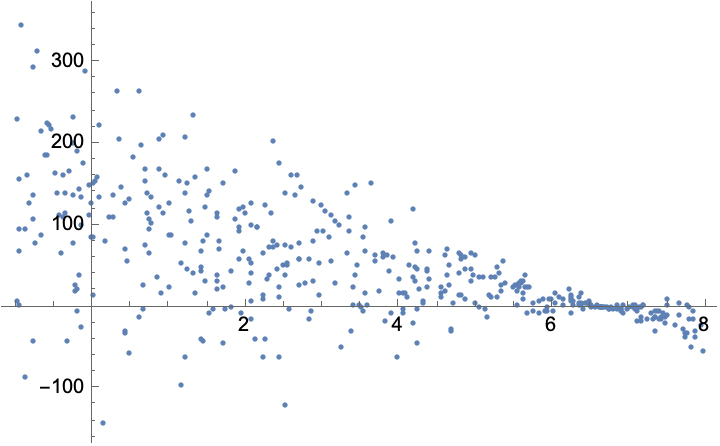
\includegraphics[width=0.9\textwidth]{reg3.png}
	   \caption*{(c)}
	\end{minipage}
	\begin{minipage}{0.45\textwidth}
	   \centering
	   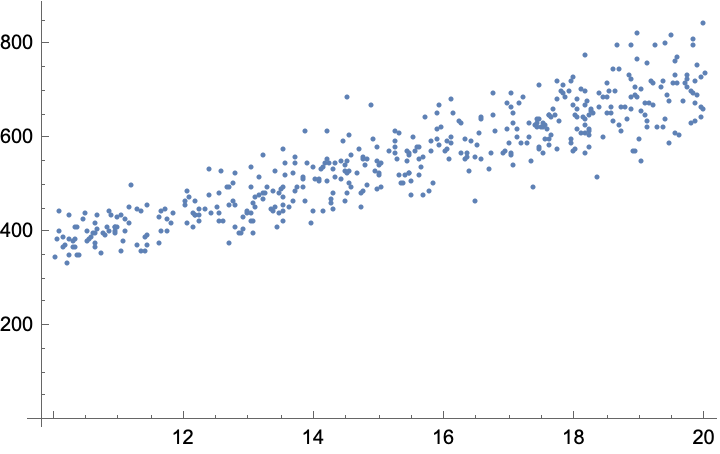
\includegraphics[width=0.9\textwidth]{reg4.png}
	   \caption*{(d)}
	\end{minipage}
	\end{figure} \pspace

\begin{enumerate}[(i)]
\item \underline{\hspace{1.5cm}}: $R= -0.9831$ \pspace
\item \underline{\hspace{1.5cm}}: $R= -0.6050$ \pspace
\item \underline{\hspace{1.5cm}}: $R= 0.4635$ \pspace
\item\underline{\hspace{1.5cm}}: $R= 0.9032$
\end{enumerate} 






% Question 3
\newpage
\question Suppose $A$, $B$, and $C$ are events in a finite probability space. Suppose $P(A)= 0.40$, $P(B)= 0.20$, $P(C)= 0.30$, $P(A \text{ and } B)= 0$, and $P(B \text{ and } C)= 0.05$. \pspace

\begin{parts}
\part[2] Assuming $A$ and $C$ are independent, compute $P(A \text{ and } C)$. \vfill
\part[2] Still assuming that $A$ and $C$ are independent, find $P(A \text{ or } C)$. \vfill
\part[2] Are $A$ and $B$ disjoint events? Explain. \vfill
\part[2] Are $A$ and $B$ independent events? Explain. \vfill
\part[2] Find $P(B \;|\; C)$. \vfill
\end{parts}



% Question 4
\newpage
\question Students across various STEM majors at local colleges were surveyed to determine whether they preferred Netflix, Hulu, Disney$+$, or HBO Max. The results are shown below.
	\begin{table}[!ht]
	\centering
	\begin{tabular}{|r||c|c|c|c|c||c|} \hline
	& Biology & Chemistry & Computer Science & Physics & Mathematics & Total \\ \hline\hline
	Netflix & 3 & 7 & 14 & 4 & 8 & 36 \\ \hline
	Hulu & 6 & 13 & 12 & 3 & 7 & 41 \\ \hline
	Disney$+$ & 15 & 4 & 1 & 4 & 2 & 26 \\ \hline
	HBO Max & 10 & 2 & 5 & 2 & 1 & 20 \\ \hline\hline
	Total & 34 & 26 & 32 & 13 & 18 & 123 \\ \hline
	\end{tabular}
	\end{table}

\begin{parts}
\part[2] What is the probability that a randomly selected student was a Physics major that preferred Disney$+$? \vfill

\part[2] What is the probability that a randomly selected student preferred Hulu? \vfill

\part[2] What is the probability that a randomly selected student preferred Netflix or was a Chemistry major? \vfill

\part[2] What is the probability that a Biology or Computer Science major preferred Netflix? \vfill

\part[2] What is the probability that a student that preferred HBO Max was a Mathematics major? \vfill
\end{parts}



% Question 5
\newpage
\question Twenty-three students in a middle school class were asked whether they had any pets. Of the students, eight said that they had a dog, five said they had a cat, and two students said that they had both. \pspace

\begin{parts}
\part[3] What is the probability that a randomly selected student did not have a dog or cat? \vfill

\part[3] What is the probability that a randomly selected student had a dog or a cat? \vfill

\part[4] Assuming that a student with a cat was randomly chosen, what is the probability that they have a dog? \vspace{6.7cm} \vfill
\end{parts}



% Question 6
\newpage
\question When it comes to `fine' Mexican dining, people agree the two best options are Chipotle or Moe's. One survey suggested 80\% of people prefer Chipotle to Moe's. However of those surveyed, only 40\% of people that went to Chipotle had a good experience whereas 60\% of Moe's customers had a good experience. \pspace

\begin{parts}
\part[3] What is the probability that a randomly selected person had a good experience at Chipotle or Moe's? \vfill

\part[3] What is the probability that a randomly selected person either preferred Moe's or had a bad experience at Chipotle? \vfill

\part[4] What is the probability that a person that did not have a good experience had it at Chipotle? \pvspace{6.3cm} \vfill
\end{parts} 



% Question 7
\newpage
\question ``Step right up,'' yells a clown at a carnival. ``Try your luck and see if fortune favors you today!'' You walk up to the booth. The clown explains that you can pay \$1 to try your luck at a dice rolling game. If you roll either a one, two, three, or four, you win nothing. If you roll a five, you receive \$0.50. However, if you roll a six, then you win \$5. \pspace

\begin{parts}
\part[7] Compute the amount, on average, you can expect to win playing this game. \vspace{5cm} \vfill

\part[3] In the long run, should you play this game? Explain your reasoning using your computation in (a). \vfill
\end{parts}



% Question 8
\newpage
\question High school students looking to go to college will often take either the SAT or ACT. The ACT parent company data suggests that ACT scores in New York State were normally distributed with mean 26.3 and standard deviation 2.3. \pspace

\begin{parts}
\part[3] What percent of students in NYS receive below 23.2 on the ACT? \vfill

\part[3] What percent of students in NYS receive above 32.7 on the ACT? \vfill

\part[3] What percent of students in NYS receive between 23.2 and 32.7 on the ACT? \vfill

\part[4] If you surveyed 80 students that took the ACT in NYS, what is the probability that their average score was below 25? \vfill
\end{parts}



% Question 9
\newpage
\question There are a plethora of quick dining options in the United States. A recent survey approximates that 1 in 5 people have been to a Sonic drive-in. Suppose that ten people are randomly surveyed. \pspace

\begin{parts}
\part[3] What is the probability that exactly three of them had been to a Sonic before? \vfill

\part[3] What is the probability that less than four of them had been to a Sonic before? \vfill

\part[3] What is the probability that at least one of them had been to a sonic before? \vfill

\part[4] Using the normal approximation to the binomial distribution, approximate the probability that if 300 people were surveyed that less than fifty of them had been to a Sonic before? \vfill
\end{parts}


\end{questions}
\end{document}